\section{ATLAS Detector}
\label{sec:ATLAS}

A Toroidal LHC ApparatuS (ATLAS) is a general-purpose detector of LHC that detects events from proton-proton, and heavy ion collisions \cite{ATLAS}. It is $44$ meters long and $25$ meters wide cylindrical-shaped detector built around LHC Interaction Point 1 \cite{ATLAS}. ATLAS has multiple concentric sub-detectors layered around the beamline, providing forward-backward symmetric coverage. The two proton beams collide at the center of the detector producing outgoing particles from hard scattering, underlying events, and pile-up. The outgoing particles interact with the detector material leaving tracks and energy deposits in several layers of the sub-detectors. 

The sub-detector closest to the beamline is the \textit{Inner Detector (ID)}, which measures the trajectories of the charged particle and plays a crucial role in identifying the physical position of the hard-scattering, also known as the \textit{primary or hard-scattering vertex}. The ID is surrounded by a solenoid magnet that provides a $2$ T magnetic field to bend the particle trajectories for momentum measurements \cite{ATLAS}. Outside the solenoid lies the \textit{electromagnetic calorimeter (ECAL)} and then the \textit{hadronic calorimeter (HCAL)}, which measure the energy of electromagnetic and hadronic physics objects, respectively. The outermost layer of the ATLAS detector is the \textit{Muon Spectrometer (MS)} that identifies the muons and provides a secondary measure of their momentum. The MS is embedded inside a toroidal magnetic field that provides a magnetic field up to 3.5 T \cite{ATLAS}. Figure \ref{fig:ATLAS} shows a schematic of the ATLAS detector with all its sub-detectors.

\begin{figure}[!htb]
    \centering
    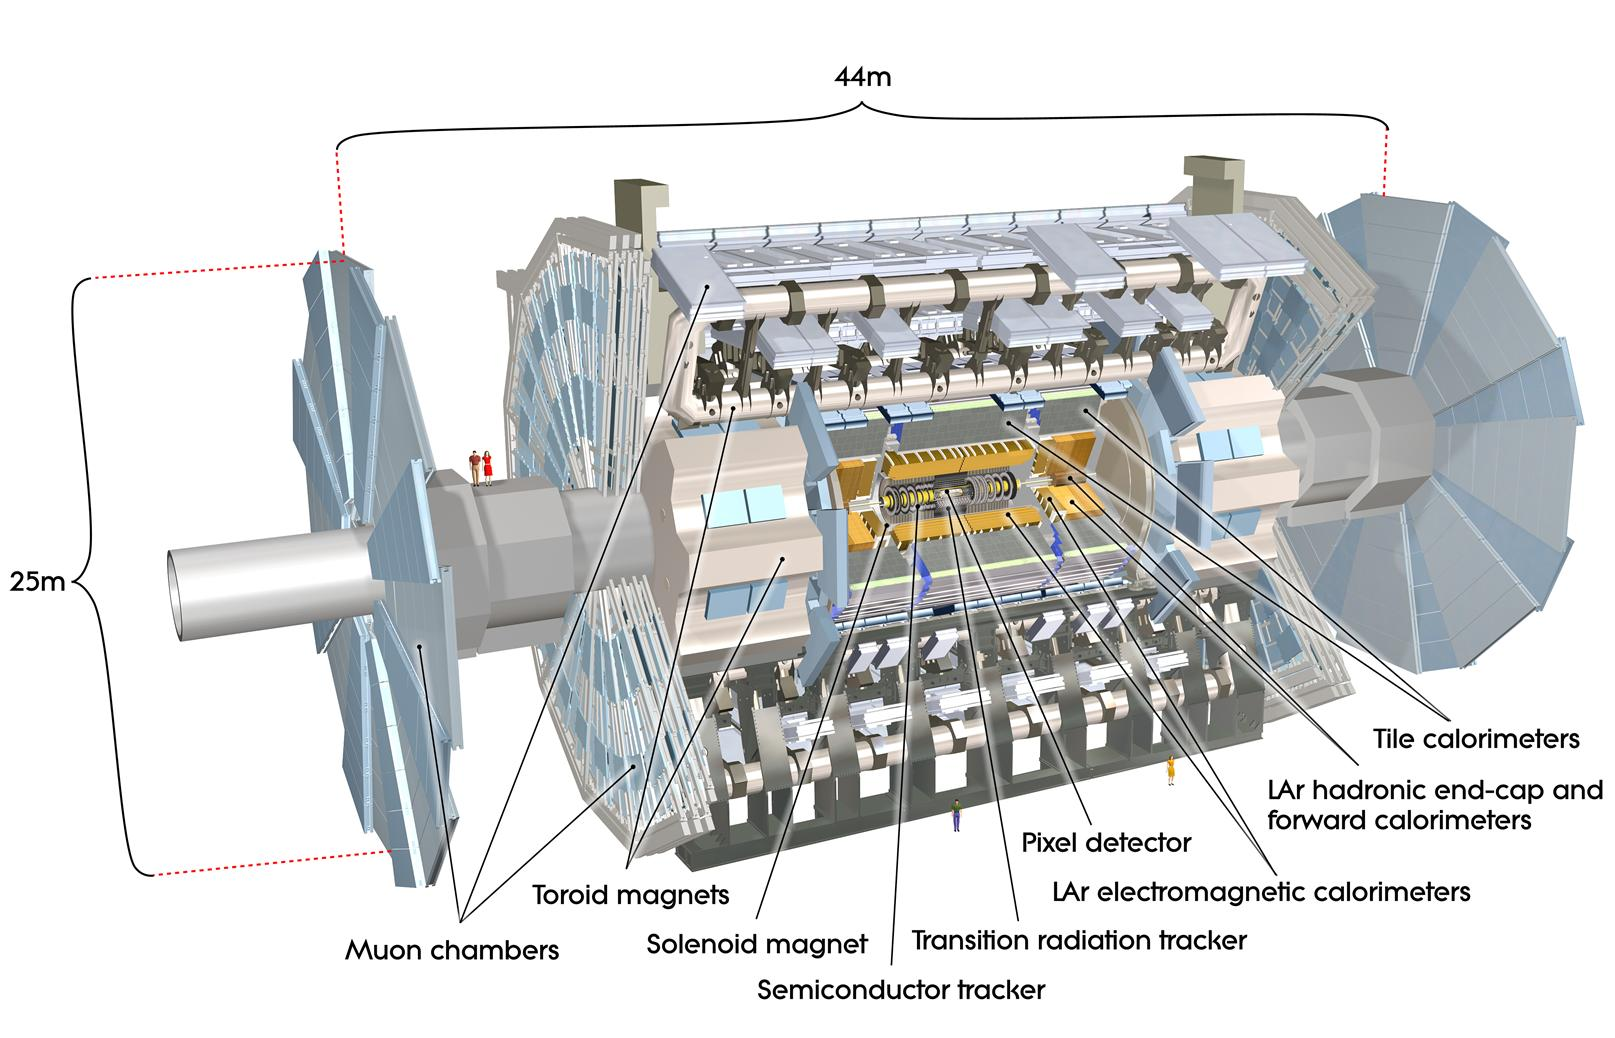
\includegraphics[width=.98\linewidth]{figures/LHC/AtlasDetector.png}
    \caption{ A detailed schematic of the ATLAS detector with all its sub-detectors \cite{ATLAS}.\label{fig:ATLAS}}
\end{figure}

\subsection{ATLAS Coordinate System}
\label{subsec:ATLASCS}

ATLAS measurements use a right-handed coordinate system with the nominal interaction point as the origin. The beamline is along the cylindrical symmetry axis of the detector, which defines the longitudinal \textit{z}-axis. The transverse \textit{xy}-plane is perpendicular to the beam direction, where \textit{x}-axis points to the center of the LHC ring and \textit{y}-axis points upwards towards the surface. Figure \ref{fig:ATLAS_CS} shows a schematic of the ATLAS coordinate system. The angle measured around the beamline in \textit{xy}-plane gives the azimuthal angle $\phi$, whereas the angle measured with respect to the \textit{z}-axis gives the polar angle $\theta$. Transverse momentum ($p_{T}$) is particle's momentum in the \textit{xy}-plane, defined as 
\begin{equation}
p_{T} = \sqrt{p_{x}^2+p_{y}^2}=p\sin\theta.
\label{eqn:pT}
\end{equation}
\textit{Rapidity (y)} defined in terms of a particle's energy ($E$) and momentum ($p$) is a commonly used collider physics quantity defined as, 
\begin{equation}
    y = \frac{1}{2}\ln{ \left( \frac{E+p_{z}}{E-p_{z}} \right) }.
    \label{eqn:Rapidity}
\end{equation}
Particles with larger momentum along the \textit{z}-axis have larger values of rapidity, whereas particles with larger momentum values in the transverse plane have smaller values of rapidity. For particles with negligible mass, the rapidity approaches a purely angular variable called \textit{pseudorapidity ($\eta$)} defined as
\begin{equation}
    \eta = \frac{1}{2}\ln{ \left( \frac{ |\vec{p}|+p_{z}}{ |\vec{p}| -p_{z}} \right) } = -ln { \left[ \tan \left( \frac{\theta}{2}\right) \right] }. 
    \label{eqn:PseudoRapidity}
\end{equation}
Higher values of rapidity and pseudorapidity refer to the forward region of the detector. The ATLAS detector has full coverage in $\phi$ and coverage up to $|\eta| < 4.9$, corresponding to $1.3^{\circ} < \theta < 178.7^{\circ} $ \cite{ATLAS}. 

\begin{figure}[!htb]
    \centering
    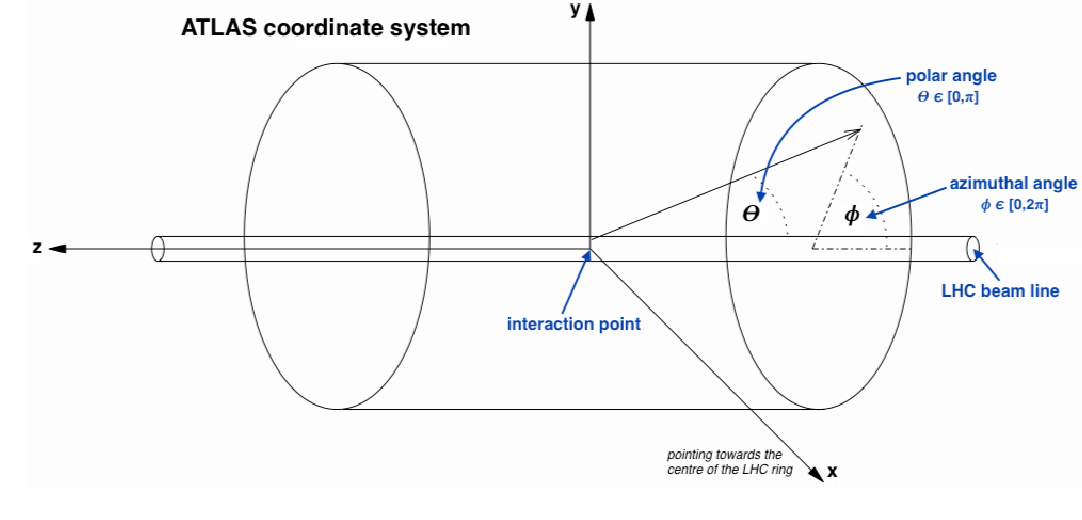
\includegraphics[width=.98\linewidth]{figures/LHC/ATLAS_CoordinateSys.png}
    \caption{ A schematic of the right-handed ATLAS coordinate system \cite{ATLAS_CoordSys}.\label{fig:ATLAS_CS}}
\end{figure}

\subsection{Inner Detector}
\label{subsec:ID}
The inner detector is the innermost sub-detector of ATLAS and is responsible for tracking charged particles' trajectories and identifying the hard scattering vertex. Closest to the interaction point is the Insertable B-Layer (IBL) \cite{ATLAS_IBL}, which was installed between Run-1 and Run-2 to improve tracking at higher pile-up. The IBL is highly granular, consisting of roughly 12 million silicon pixel sensors with a size of $50\times 250 ~\mu m^2$ \cite{ATLAS_IBL}. Located $3.3$ cm from the beamline, the IBL can reconstruct tracks with $|\eta|<2.5$ \cite{ATLAS_IBL}. 

Three layers of silicon-pixel detectors for a total of $1,744$ pixel sensors, each with pixels of size $50\times 400 ~\mu m^2$, surround the IBL \cite{ID_Pixel}. The slightly larger pixel size compared to the IBL is optimal for the pile-up at a distance larger than $5$ cm from the interaction point. The pixel detector provides coverage up to $|\eta|<2.5$ with a single point spatial resolution between $5$ and 12 $\mu$m \cite{ID_Pixel}. Surrounding the pixel detector is the Semiconductor Tracker (SCT) consisting of five layers of silicon microstrip detectors with a mean strip pitch of $80 ~\mu m$ in the barrel region, and varying pitch of  $57-94 ~\mu m$ in the end-cap regions \cite{ID_Strips}. 

At a distance about $50$ cm from the beamline lies the outermost layer of the ATLAS inner detector, the Transition Radiation Tracker (TRT), with $370,000$ straw tubes each with a diameter of $4$ mm \cite{ID_TRT}. Each TRT straw tube is filled with an Argon-based gas mixture and has a $31~\mu m$ diameter tungsten wires \cite{ID_TRT}. 

Figure \ref{fig:ATLAS_ID} shows the different parts of the inner detector and their distances from the interaction point.

\begin{figure}[!htb]
    \centering
    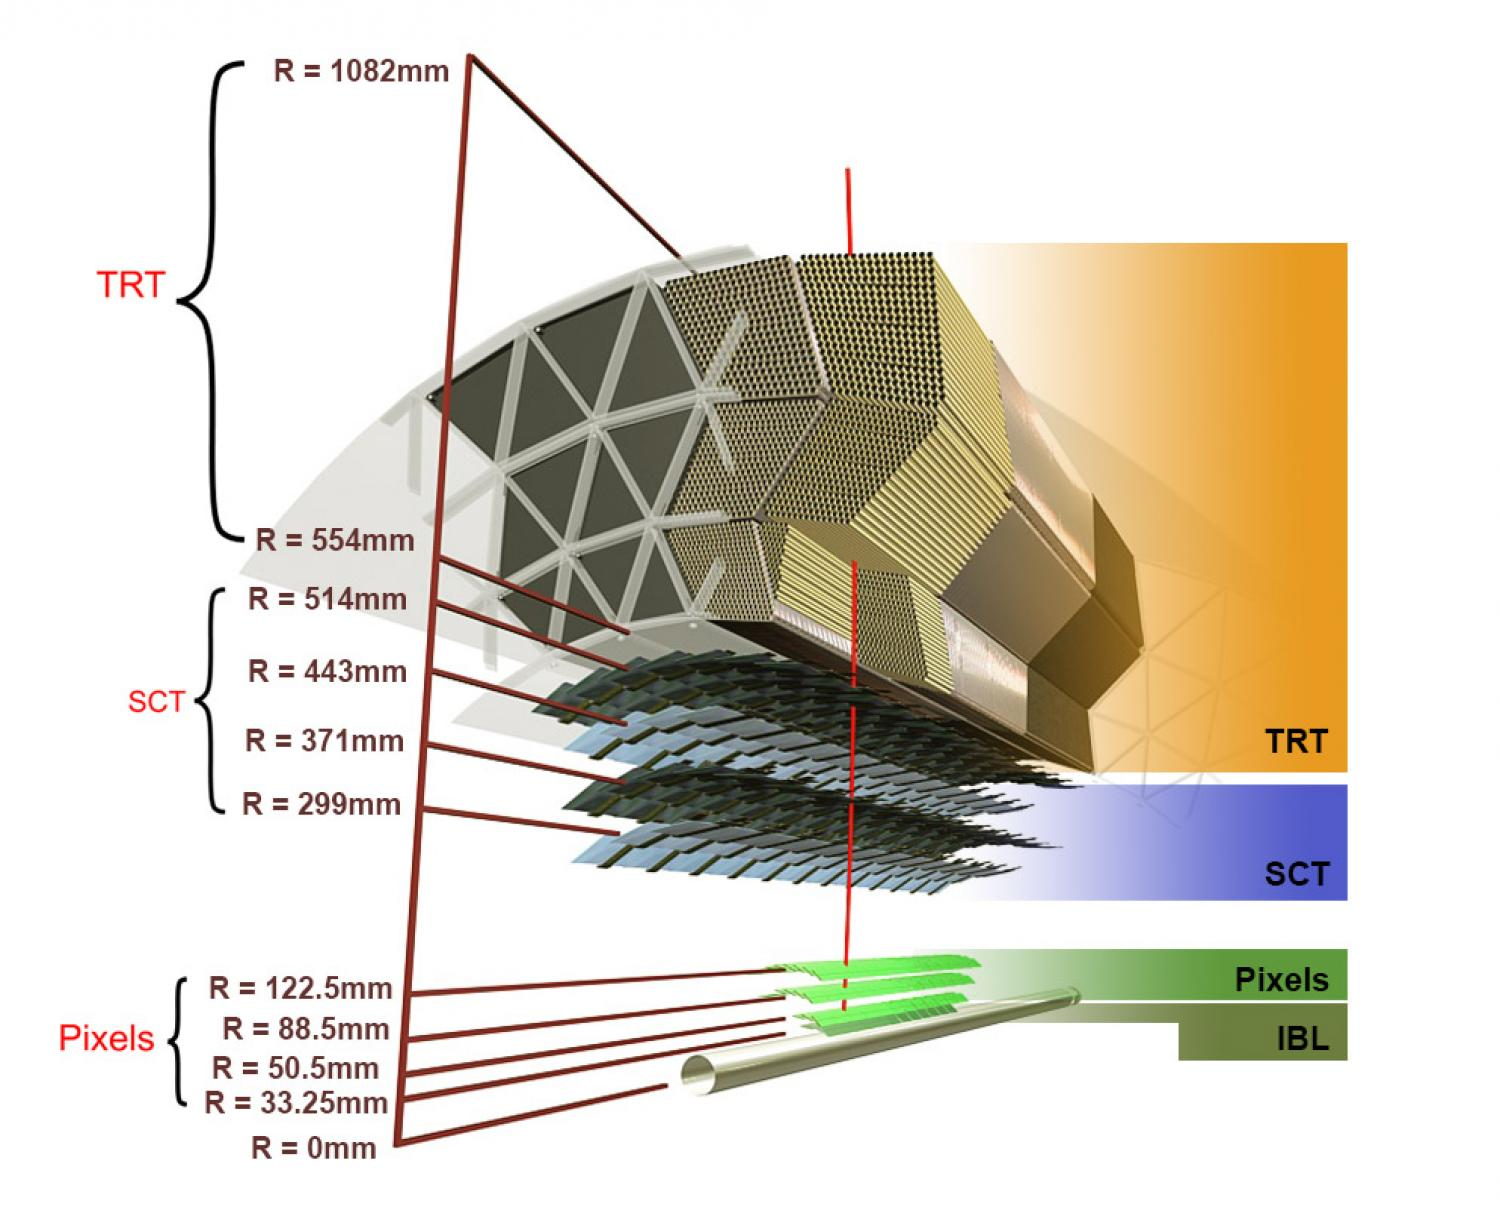
\includegraphics[width=.98\linewidth]{figures/LHC/ATLAS_InnerDetector.jpg}
    \caption{ A schematic of the inner detector of ATLAS showing the IBL, pixel detectors, SCT, and TRT \cite{ID_Align_Run2}.\label{fig:ATLAS_ID}}
\end{figure}

\subsection{Calorimeters}
\label{subsec:Cal}

ATLAS has two calorimeters, electromagnetic and hadronic, designed to measure the energy of charged and neutral particles up to $|\eta|\leq4.9$ \cite{ATLAS}. When interacting with a material, an electron loses its energy by photon emission, producing a pair of oppositely charged electrons, which could each radiate a photon, creating an electromagnetic shower in the detector. Similarly, in the hadronic calorimeters, the hadronic particles also result in a shower of particles through multiple scattering. The calorimeters measure the energy of the particles by reconstructing the electromagnetic and hadronic showers. The calorimeters are designed to fully absorb the shower of all particles except muons and neutrinos. Thus, materials with high radiation length ($X_{0}$) and high interaction length ($\lambda$) are chosen respectively to build the electromagnetic and hadronic calorimeters.

The accordion-shaped electromagnetic calorimeter lies outside the solenoid surrounding the ID consisting of an alternate layer of lead absorber plates and highly granular liquid-argon (LAr) cells to precisely measure the energies of electrons and photons. It comprise of one barrel section in $|\eta| < 1.475$ region and two end-caps in $1.375 < |\eta| < 3.2$ region \cite{ATLAS_ECAL}. The calorimeter's central region ($|\eta| < 2.5$) is designed to identify electrons and photons with high precision.

The hadronic calorimeter surrounds the ECAL and consists of steel absorbers and active scintillator tiles in $|\eta| < 1.7$ region. The end-cap regions ($1.5 < |\eta| < 3.2$) consist of copper absorbers and active LAr detectors. The forward region ($3.2 < |\eta| < 4$) comprises the tungsten absorber followed by active LAr detectors \cite{ATLAS_HCAL}. 

Figure \ref{fig:ATLAS_Cals} shows the layout of the ATLAS calorimeters. The calorimeters are segmented into cells which consist of an alternating layer of passive materials to absorb the particle and active layers to measure the energy. Object reconstruction in calorimeters starts with the formation of \textit{topological clusters} of cells with significant energy deposits.

\begin{figure}[!htb]
    \centering
    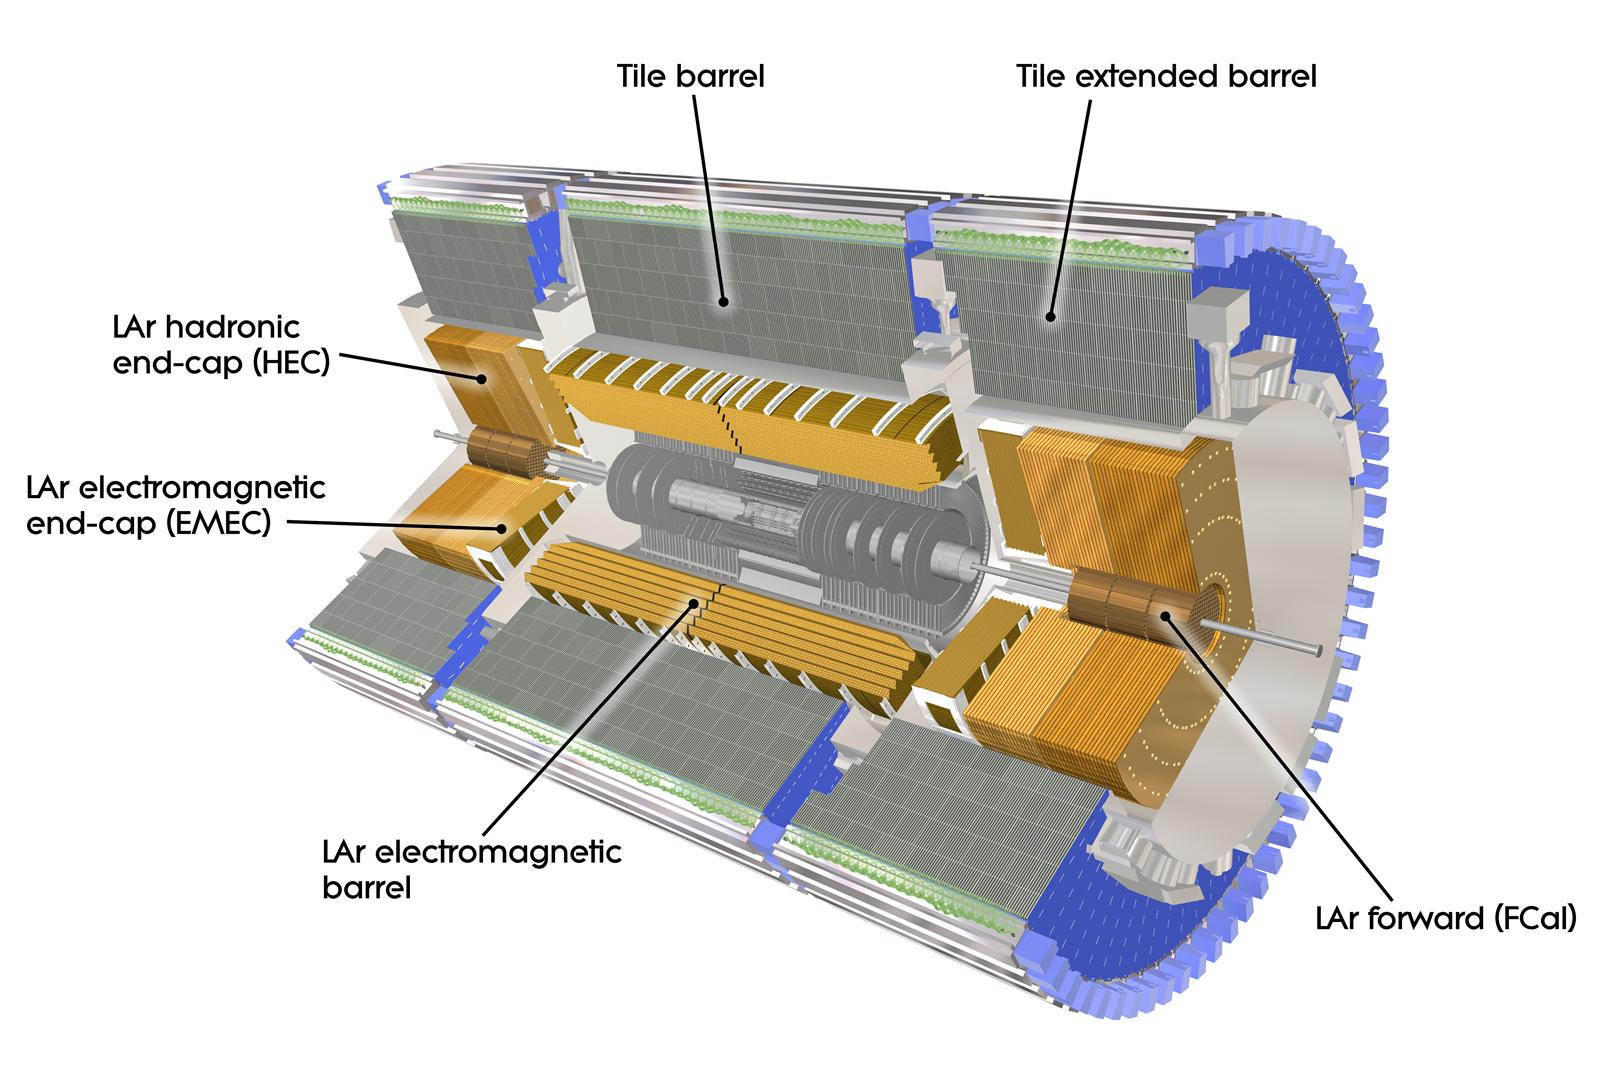
\includegraphics[width=.98\linewidth]{figures/LHC/ATLAS_CALO.jpeg}
    \caption{ A schematic of the electromagnetic and hadronic calorimeters in ATLAS \cite{ATLAS}.\label{fig:ATLAS_Cals}}
\end{figure}

\subsection{Muon Spectrometer}
\label{subsec:MS}
Muons are deeply penetrating charged particles that leave minimum ionizing deposits in the calorimeter. The muon spectrometer, the outermost part of the ATLAS detector, identifies the muons and gives an additional measure of muon's momentum by tracking its trajectories which are deflected in the magnetic field provided by the superconducting toroidal magnets \cite{ATLAS}. The MS tracks muon with $p_{T} > 3$ GeV in $|\eta| < 2.7$ range \cite{ATLAS}. As shown in Figure \ref{fig:ATLAS_MS}, the muon spectrometer comprises four types of detectors. The three stations of Monitored Drift Tubes (MDT) occupy the $|\eta| < 2.0$ region, while the Cathode Strip Chambers (CSC) cover the $2.0 < |\eta| < 2.7$ region \cite{ATLAS}. Resistive Plate Chambers (RPC) ($|\eta| < 1.05$) and the Thin-gap Chambers (TGC) in $|\eta| = 1.05$ range comprises the trigger system in MS \cite{ATLAS}. 

\begin{figure}[!htb]
    \centering
    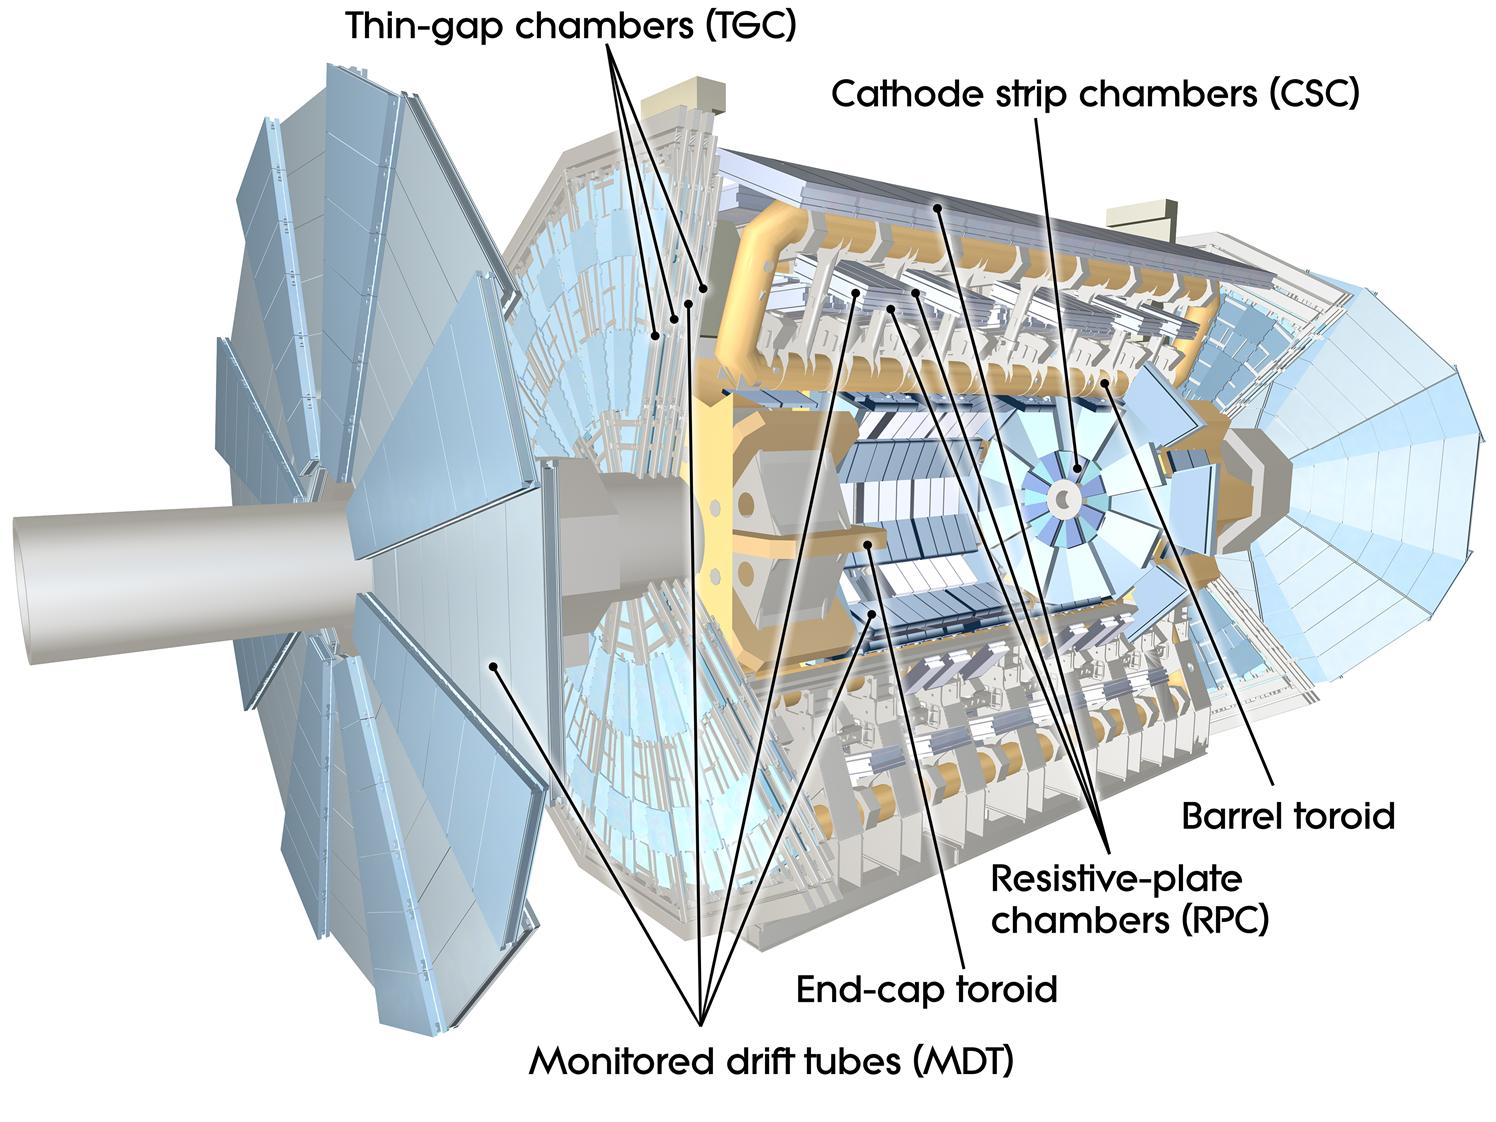
\includegraphics[width=.98\linewidth]{figures/LHC/ATLAS_MS.jpeg}
    \caption{ A schematic of the different components of the muon spectrometer in ATLAS \cite{ATLAS}.\label{fig:ATLAS_MS}}
\end{figure}